% Version with Darius's comments  = results_2.tex


\section{Results}
% Factors which shape user experience, behavior and perception.
    We present our findings 
    from a 4-weeks `in-the-wild' study 
    regarding the factors influencing self-reports of mental health and wellbeing via \ac{CA} 
    involving $20$ participants with \ac{AD}.
% quantitative data: adherence and UEQ
    first, we report on the quantitative findings of the study which includes participant's 
    adherence to the study protocol and perceived experience as measured by their response to the \ac{UEQ} questionnaire. 
% quotes and themes that represent/discuss the findings
    We then present the our findings from the thematic analysis of the interviews which shows that users' self-reporting experience is strongly shaped by
        \ac{CA} features and limitations,
        users' emotional state and attachment to \ac{CA},
        social situation, and
        their privacy perceptions.
    We discuss the findings in 4 major themes and sub-themes:
        (i) Users' tactics to overcome \ac{CA} limitations to self-reports,
        (ii) Sometimes all you need is someone who listens,
        (iii) Social situation: ,
        (iv) Privacy perceptions.
% design suggestions
    Finally, we summarize participants' \ac{CA} design suggestions to support self-reports of mental health and wellbeing.

    
    \subsection{Adherence}  
        \begin{figure}
            \centering
            \includegraphics[clip, trim=0cm 0cm 0.15cm 0cm, width=\textwidth]{figures/adherence.pdf}
            \caption{Participants' adherence to daily self-reports of mental health and wellbeing via \acl{app}.Each dot represents an entry for the day. Annotations reflect each participant's adherence rate during the study duration. The red bar indicates Dialogflow's service outage on August 20, 2020. Participants were not able to use \acl{app} on that day.}
            \label{fig:adherence}
        \end{figure}
        % \footnote{https://issuetracker.google.com/issues/165676621}
            
        Analysis of the timestamps collected through \acl{app} shows that the average participants' adherence rate to self-report was $74.64\%$, which is comparable to prior studies implementing \ac{EMA} in mobile devices~\cite{wen2017compliance}. Figure \ref{fig:adherence} illustrates the summary of the participant's adherence to daily self-reports during the study period. 
            
        The participants with lower than 60\% of adherence rate (P1, P11, P20) reasoned that they were unable to use \ac{CA} due to
            the immobility of the smartspeaker, 
            their own mental state and 
            privacy reasons. 
        P1, for example, when asked about her low adherence rate, they explained: 
        \textit{``When I am quite down, I close down. I don’t talk to anyone. It’s not just \acl{app}. During the times I was lived with my boyfriend, it was difficult for me to ask him to leave the room as I wanted privacy to talk to \acl{app}. And sometime, I wasn’t in town''}.


    \subsection{User experience}    
        \begin{figure}
            \centering
            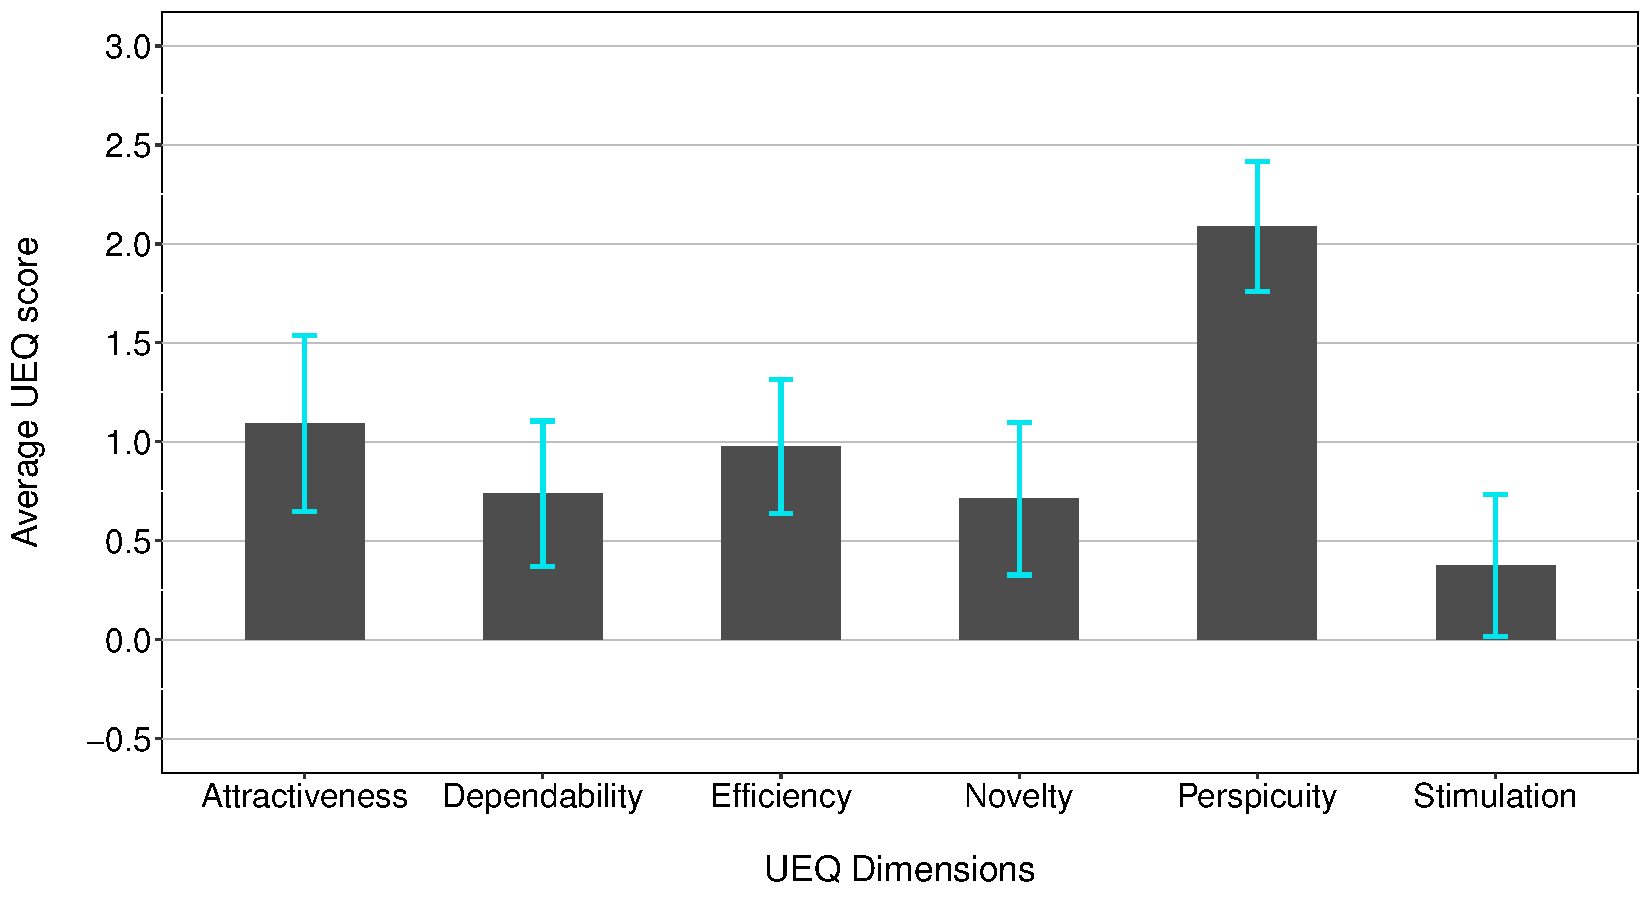
\includegraphics[clip, trim=0cm 0cm 0.25cm 0.25cm, width=\textwidth]{figures/ueq.pdf}
            \caption{Participant's mean \ac{UEQ} score in each dimension with error bars reflecting margin of error.
            Values between $-0.8$ and $0.8$ represent a more or less neutral evaluation of the corresponding scale, values $> 0.8$ represent a positive evaluation and values $< -0.8$ represent a negative evaluation.}
            \label{fig:ueq}
        \end{figure}
        
        Participant's response to \ac{UEQ} questionnaire reflects their positive experience using \ac{CA} to self-report their mental health and wellbeing. 
        Figure \ref{fig:ueq} shows participant's impression of their self-reporting experience via \acl{app} in terms of
            Attractiveness ($U = 1.09, SE = 0.44 $),
            Dependability ($U = 0.74, SE = 0.37 $),
            Efficiency ($U = 0.98, SE = 0.34 $),
            Novelty ($U = 0.71, SE = 0.38 $),
            Perspicuity ($U = 2.09, SE = 0.33 $), and
            Simulation ($U = 0.38, SE = 0.36 $).
                
        The figure illustrates participants' positive perceptions on \ac{CA}'s perspicuity and attractiveness, and indicates participant's acceptance of \ac{CA} for self-reports. 
        Participants' neutral views on dependability, efficiency, novelty and simulation of \ac{CA} self-reports suggest the \textbf{need for design and technical improvements}. 
        
        In line with prior findings~\cite{lau2018alexa, Rafal2018Workplace}, participants in this study expressed that the convenience offered by \ac{CA}'s hands-free speech-based interaction was the primary facilitator to use \ac{CA} for self-reports.
            \textit{``I think I love it because it’s like an interface you talk directly to. You can just talk to it. It’s super easy to use. You don’t have to open your laptop and go to a specific page. I can just go home, open the door and talk to \acl{app}, super easy''} [P1].
        They described that speech being a more natural form of interaction, allowed them to express their emotions freely and spontaneously compared to other forms of self-reports. 
            \textit{``Speaking is much easier because you can just let the words flow and you don't have to think about it''} [P14].
        
    \subsection{Tactics to overcome \ac{CA} limitations to support self-reports}
% limitations: don't understand user pausing and 12 sec limitation
        Participants described that \ac{CA}'s technical limitations as described in Section \ref{sec:ca_limitations}
        frequently interrupted their self-reports impairing their self-report experiences.
        % 
        \ac{CA}'s inability to recognize pauses between user utterances and the 12 second limit on user response, in particular, caused the interruptions. 
        % 
        Participants were interrupted in the middle of their self-reports by posing the following question before they have completed their responses.        
        
        \subsubsection{Effects of \ca{CA} limitations on self-reports}
% frustration
            These interruptions frustrated participants.
            % \textit{`I'm like `No bitch, you cut me off. So, shut up'..''}. [P9].
            As a result, participants often simply quit the conversation without completing their self-reports:
                \textit{``When it cut me off, I was little annoyed, I didn't have so much patience with her. I was like, Okay fine, that's it for today''} [P18].
% feeling of rejection#
            Many participants compared their \ac{CA} self-report with a human-human conversation. P8 and P9 expressed the feeling of rejection due to the repeated interruptions and the fact that they were not able to self-report their emotions fully.
                \textit{``I know it's not a human being. I know it's this little round little thing, but still it's like, I'm trying to be personal here and then you're interrupting me. It feels like a rejection''} [P9].
            They related their interrupted self-reporting experience with talking to a person who does not care. 
                \textit{``I felt like a bit like when you talk with a friend, and they don't want to listen to you''} [P8].
% disconnect
            Participants shared that it was important for them that they felt listened to or cared for, although they were aware that \acp{CA} could not understand their emotions nor care about what they shared.
                \textit{``Of course, the software doesn't care. But, you want the illusion that it cares about you''} [P5].
% value
            Because they were not able to share their thoughts completely, P3 questioned the value of self-reporting via \ac{CA}: 
                \textit{``She'll cut you off anyway. There's no point to talking to someone if you're not allowed to complete your thoughts''}.
        
        
        
        \subsubsection{Users' tactics to adapt to \ac{CA} limitations}
            Each participant was informed about the \ac{CA} limitations at the pre-study session and instructed to add multiple entries if they were unable to complete their thoughts. However, only a few participants reported adding multiple entries. 

% participants who added multiple entries 
            Participants who self-reported adding multiple entries, accepted the \ac{CA} limitations and sympathized with the technology. Despite the frustrations, they followed the instructions without implementing any of their own tactics.
                \textit{``With my frustration, I took a deep breath and thought it’s just a technology. It’s in it’s starting phase - I let it do it’s thing''} [P3].
            P12 compared \ac{CA}'s 12-second limitation with human's limitation to listen to someone, quoting,
                \textit{``I guess that there's also like a limit to how, how long she can listen, like another person would also have''}.

% participants who implemented their own tactics (why no multiple entries?)
            In contrast, participants who refrained themselves from self-reporting in multiple sessions described that they lost the train of their thoughts by the time they are ready for an additional session. P9 stated,
                \textit{``I tried to do that, but the problem is that you use your momentum or train of thought when you're interrupted like that''}.
            P2 perceived their conversation with \acl{app} like human-human conversation and thought that it would be rude to ask \acl{app} to listen to them again:
                \textit{``I don't think I did [multiple entries], because when you're done talking to her and she is like `Thanks for sharing that. Have a nice day'. And then it would feel rude to ask her again and then tell her about the day again. I didn't want to bother her more than once''}.
            Others explained that limitations affected their self-reporting experience mainly at the beginning of the study they were able to adapt to the \ac{CA} constraints and eventually learned to talk to the \ac{CA}.
                \textit{``It was kind of hard in the beginning as she is really sensitive to pauses and doesn't give you any space to think. But my brain adapted that really quite quick''} [P7].
%tactics 
            In order to adapt to the \ac{CA} limitations they implemented tactics such as (i) changing their natural way of talking and (ii) formulating self-reports beforehand.
            
            \subsubsubsection{\textbf{Changing the natural way of talking. } }
            Participants who change the way they naturally talked, stretched their utterances, used filler words, and talked faster or shorter. 
                \textit{``I tried different tricks like for instance I tried to make some songs like `hmmm...leeeet meeee thiiiiink...' but it seems like my process was too slow for \acl{app}. So at one point, I started giving very short answers so I won’t be cut off yet could answer''} [P1].
            Participants viewed this tactic as a compromise to their natural way of talking as remarked by P8:
                \textit{``My speech is a bit artificial, not very smooth, and didn't feel fluent. I had to change the way I talk to fit what \acl{app} can accept}.''
                
            \subsubsubsection{\textbf{Formulating self-reports beforehand. } }
            Those who formulated their self-reports before talking to the \ac{CA}. P16 for example, divided their response into three segments to match \acl{app}'s dialog design:  
                \textit{``I realized, okay two sentences for the first question, two sentences for the second question, and one sentence for the last question. Just five sentences overall''}.
            
            Participants stated that the process of formulating the self-reports before talking to \ac{CA} helped them reflect on their day. P11 viewed the process meditative, quoting, 
            \textit{``It helps you organize things in your head. And also, I believe it's like a form of meditation. It's like `you time', you know, I believe it helps you clear your mind''}.
            % 
            P6 compared their experience writing a diary and mentioned that the process of preparing the response to talk to \ac{CA} allowed them to better reflect and emphasize on their day: 
                \textit{``It's not just three pages of how I saw something nice and I had a nice cup of coffee....It really is an emphasis on three things which really matter to me''}.
            % 
            In contrast, P7 perceived the that tactic minimized their control over the interaction, although they were able to mitigate the limitations:
                \textit{``I started thinking about what I want to say before I called her up. Normally, when people talk about feelings, they need space and time for pauses. I knew my \acl{app} friend could not really do that. So we had to do it on her terms''} [P7].
            % 
            In some cases, participants expressed that their self-reports were often shallow because they presumed that they would not have enough time to express their feelings entirely.
                \textit{``She expects an answer in few seconds, so I'll be like, `tired', `decent', `Not sure'. So in that sense, the answer might be a bit less thought out''} [P2].   
            
            %desire to talk longer
            While participants were able to alleviate \ac{CA} limitations to self-report about their mental health and wellbeing, they expressed their desire to be able to talk for more than 12 seconds and wished that \ac{CA} did not interrupt the conversation by cutting them off mid-sentence, allowing them to reflect on their day and fully express their state of mind.        
                \textit{``I think it would make more sense if I could speak at length, and she didn't cut me off''} [P4].


    \subsection{``Sometimes all you need is someone who listens''}
% Reasons why they want someone who listens
% People want solve their problems
        Participants described that it is often challenging for them to communicate their feelings to others, including their friends, loved ones in the family or health professionals. 
        They said that listeners are often too keen to solve their problems when they express their emotions and want them to explain their situation. 
            \textit{``When you say you feel sad and empty, you don't really want the focus to be on describing how emptiness feels. You just want to say, `I'm feeling sad' and you want someone to say, `Oh, I hear you. That's okay'...''} [P6].
                
                
        
        Participants explained that they often share their thoughts and feelings to vent their emotions and not to find a solution. 
        

        They added that they strive for \textit{``emotional support instead of emotional counseling''}, as stated by P7. Participants perceived that talking to \ac{CA} about their emotions fulfilled those needs.
            \textit{``It sounds a bit stupid to say but I could say that I'm glad someone listens, except you know there isn't actually someone that listens. But it feels like it. Or at least I get to get some stuffs out. If you just need someone to vent out, you can with \acl{app}... and sometimes all you need is someone who listens than have an answer...because there's not necessarily anything to solve, you just need someone to share your thoughts and feelings so that you are not alone''} [P2].
    
        \ac{CA}'s potential for emotioniusal support was widely shared by the participants during the interview. Participants often personified \acl{app} by comparing their experience talking to \ac{CA} with their prior experiences and discussed \ac{CA}'s potential as a companion. 

        \subsubsection{Sofia a good listener}
        
        Participants characterized self-reporting their emotions via \ac{CA} as a way of emotional venting as it allowed them to express their emotions without any judgment, repercussions or unwanted solution. 

% No unwanted solution 
            Many participants shared that they often do not need a solution to their problems. Due to their mental conditions' chronic nature, they know how to cope with the situation or overcome their mental state. Therefore, they valued being heard than having their problems solved. They perceived \acl{app} as `someone' that made them feel heard -- a quality that is fundamental for sustainable long term \ac{CA}-user relationship.
                \textit{``It sounds a bit stupid to say but I could say that I'm glad someone listens, except you know there isn't actually someone that listens. But it feels like it. Or at least I get to get some stuffs out. If you just need someone to vent out, you can, with \acl{app}''} [P2].
%No judgment
            P4 For example, compared their experience sharing their feelings with humans and talking to \acl{app}. They expressed that they liked the fact that they were not judged, quoting,
            % \begin{quote}
                \textit{``I think, you cannot compare it to this conversation with someone, of course, which is more comfortable I would say. But in some way, it's really nice because you don't get advice like from people, because I know that's especially if I share that I'm quite stressed, then people say like, `Oh, then you have to, you know, go home a bit earlier' or 'You can do this' and, and of course that's not really working for anxiety in like those kind of problems so it can be quite nice to just have no judgments or something like that which I really liked about it (\acl{app}).''}
% No repercussions
            Participants also expressed that not having to think about the repercussions of the listener's reaction, their interest in the subject matter, or their feedback provided a safe space for them to vent out their emotions. P14 said,
                \textit{``It was very easy for me to talk to \acl{app} because it's like someone that doesn't, I mean, if you talk to a human, it can sometimes be that you can feel that they are not interested or may be you don't want to give them all your problems so to say, and with something like this [\acl{app}] it's quite easy because it's like a computer right so you don't have to think about someone else's feelings in this way...And for me, it's just nice to talk to someone that doesn't really bother about what I say''}.



% compassionate feedback
            Likewise, P6, who suffers from schizophrenia, expressed that they would appreciate a compassionate feedback rather than any help from people or through \ac{CA} when they have episodes like auditory hallucinations.
                \textit{``I suffer sometimes from auditory hallucinations where I like hear voices. And sometimes when I'm like in a room, working on projects. Sometimes I have to tell people like `I'm sorry. I'm distracted right now. I'm having a small episode. Please don't mind it'. And people really really want to help, and they want to understand. But it's just not what you need in that moment. You just need someone to say `Okay. That's okay. You feeling something and that's okay', `You're experiencing something and that's okay'. Because when you have a diagnosis like this, you also know that talking doesn't make it go away, but sometimes getting assurance `Okay, it's okay to feel, it's okay to experience what you experienced', that helps a lot. And in that regard \acl{app} doesn't ask, she doesn't require you to explain anything. She just asks you how are you feeling. And if you want to tell them more you can tell them more and if you don't want to, you can just say I'm feeling sad, and that's it. In that aspect, she is a listener. Sometimes a listener is exactly what you need in a situation like that''}.

% approachable
            Due to the \ac{CA}'s affordance of this trustworthy conversation, participants found \ac{CA} more approachable than human counterparts. They perceived \ac{CA} as a harmless machine that cannot turn against them no matter what they shared with it. P7 said,
                \textit{``I have massive trust issues. You know, it's probably about my upbringing. You know, I come from a family where I was not exactly allowed to be myself. I was not exactly listened to. So it's when you when you live in that condition for so many years, you kind of like grow up thinking that, you know, whoever you tell anything to they will use it against you. And so it's kind of like a self guarding mechanism. But you know, since I know that \acl{app} is a machine, she doesn't really think that much of herself and she's just there sitting on my table. That kind of makes it a little bit more approachable''}.

        \subsubsection{Companionship}
% companion
            During the interview participants discussed \ac{CA}'s value as a companion, especially when they are depressed and socially deprived. P1 described that they tend to get restrained from their social circle when they are depressed, and mentioned that \acp{CA} could in some extent be useful to fulfill the social deprivation:
            % 
            % \begin{quote}
                \textit{``When you are depressed, your social circle tends to restrain more and more. So, you’ve less opportunity to talk to someone. I like the feeling, even though \acl{app} is not so clever, I felt like I was talking to someone even though \acl{app} is not very smart. Just because of this feeling, I think it is very useful for people with depression.''}

            P5 said that \ac{CA}'s quality of being available all the time makes it a useful tool that could help them vent out their feelings when they needed, quoting,
            % \begin{quote}
                \textit{I do have friends to talk to. But, it can be a good tool. It’s always there when you need it. A friend could be busy. So, when you need to talk it out, it’s in your reach even though it’s a machine. And that can be very useful to many people. I don't think they will replace people but I think they will both exist at the same time - talk to a machine as well as a person.'' }
           
% loneliness
        In contrast, P4 stated that talking to \ac{CA} about their emotions made them feel lonely as the \ac{CA} could not understand their feelings:
        % P4 stated that talking to \acl{app} made them feel lonely.
            % \begin{quote}
                \textit{
                % Yeah, I don't know, it's like because would you would you want to talk to another machine, because something I wanted to remark on was also that 
                ``Sometimes she made me feel a bit lonely, somehow, because 
                % you're just If you want, if your intention is to have some kind of connection with another entity or something because it just you, you're the attention is to use her as somehow in therapy, and like, 
                you're just reminded that you're talking to a machine, who has no capacity to understand what you're actually feeling.''} 
                % And so it creates this longing for just another human being who can just like nod and ask dumb questions, even, you know, even if they're less qualified than a therapist or something, it's just, you know, at least they react to you.
                % 

        Further, they expressed that they are reminded that they do not have anybody to share their thoughts and feelings. Having a \ac{CA} that mimics human-like interaction makes them even lonelier because they know that it is not a human being. Therefore, they wanted \ac{CA} to be less human-like. They quoted,
            % \begin{quote}
                \textit{``The more mechanic function, I feel like its fine. And because I'm not expected, like, I don't have the expectations of meeting another thinking, feeling being. And then it's actually fine because I know I'm just like it's just me and my thoughts and that's okay. But yet you're kind of reminded that it's not that you're alone when you, when you meet something that kind of tries to mimic a human being. But isn't ... you know ... it's not convincing.''
                }
                % [P4]
                % i11
            % \end{quote}

        \subsubsection{Personification}
% Why+How they personified
        Participants personified \acl{app} in different forms such as elderly woman, dog, friend, diary person, and therapist.
        They stated that even though they were aware of the fact that the interaction between them and \acl{app} is not a conversation, the anthropomorphic characteristics of the \ac{CA} including a name and voice gave them an impression of a conversation.
        P10 who personified \acl{app} as a friend said,
                \textit{``I think, again it's the whole, having a voice and having a name, I keep referring to her as an her. Instead of, instead of it, even though it is, I'm aware of that it's, you know, it's a system. It's, it's not a person but there's something, I don't know, something happens. And I think that whole shift inside me makes me think more of her as a friend.''}
            For P9, \acl{app}'s informal language of conversation gave them a human-like impression and mentioned that overly polite language in self-report technology makes them feel the interaction unnatural.
                \textit{``I guess the tone of voice of course you can hear it's like a bit robotic, but it's not super robotic and the whole, for example, `Go ahead [P9's first name], I'm listening', that's something which is a bit more of a human way of saying things instead of being overly polite as some, some of these tools sometimes are. Sometimes I just get the idea that whenever people make these kind of technologies they make them overly polite, sort of in a way it's unnatural.''
                }
            
            P14 viewed \acl{app} as an older friend as it enabled them to reflect on their mental state and gain insights. They also mentioned that it could be either their age or \acl{app}'s voice that reminded them of someone older, remarking:
                \textit{
                ``Its more like a friend, but like for me, an older friend. It's more experienced in life. I just have the feeling that maybe \acl{app} knows more about things in life than I do. When I talk to her, I come to my own insights...the fact that I get these insights, she gives me these insights, but actually, I give them to myself. That's why I think, she is at least, she feels older to me. But I mean I'm also quite young, I'm 25 so maybe that's why.Maybe it's also just the voice or something that reminds me of someone a bit older than I am, I don't know.''
                }
            P20 expressed that talking in itself makes \acl{app} human-like. They further mentioned compared writing a diary and talking to \acl{app} by quoting,
                \textit{``You get the impression that you’re talking to someone, which is a very different feeling - you feel like you’re not talking to yourself, you feel like you’re talking to someone else. I think it’s really nice to hear a human voice saying `Tell me about your felings'. It just makes you feel like you’re talking to an imaginary person. When you're writing a diary - you’re writing for yourself.''}
            P15 compared \acl{app} to their dog with which they shared their feelings while they were upset and perceived it as as a `talking diary'.
                \textit{``You know what I compare \acl{app} to? I just realized that ... to my dogs. Because a lot of the times, especially when I was growing up, if I was upset I went outside sat down and talked to my dog and I was just petting the dog who had no freaking clue what I was talking about, and did not care at all. And it made me feel better...the dog will sit down and listen and has no reaction or anything, and it's so good.''}
            
% Personification and self-reporting behavior
            We found that participants' experience with \ac{CA} shaped how they personified \ac{CA}, and it had a profound effect on their self-reporting behavior.

            % +ve
            Participants shared that since they perceived \ac{CA} like a person, they did not want to share just the negative emotions. They felt the need to share positive emotions as well. 

            P2 justified the positive attitude towards \ac{CA} as human decency, quoting,
            % -ve
            Few participants found \acl{app}'s conversational skill primitive negatively affecting how they personified \acl{app} and their self-reporting experience.
            % 
            Referring to the time limitation under which they have to respond to \ac{CA}'s question, limited variation of questions and the tone of \ac{CA}'s voice, P3 personified \acl{app} as an impatient old lady, remarking,
                \textit{``\acl{app} is a very impatient woman and she’s probably quite old because she stops - she’s very monotoned, there’s no variation.''
                }

            P9 described that they had an annoying self-reporting experience with \acl{app} and that they felt rejected talking to the agent. They personified the agent as friend who does not care:
                \textit{``One of the reasons why it would annoy me was that it kind of feels a bit like a rejection. When, like, okay now I'm actually sitting down trying to share something personal. I know it's not a human being. I know it's this little round little thing, but still it's like, I'm trying to be personal here and then you're interrupting me. `Shut up'. It's kind of like that, you know, that friend who like sits with the phone when you try to talk, talk about something deep, like yeah ... okay fine ... just say you don't want to listen to me.''}
       
        
        \subsubsection{Emotional venting}
    % releasing repressed emotions
            Some participants considered talking to the \ac{CA} about their mental state an effective way of emotional venting, which is regarded as an effective way of finding relief by releasing strong or repressed emotions~\cite{bennett1991irrationality, tonnaer2020explosive, leslie2008boxing}.
                \textit{``I almost see it as, you know, when you get super upset, you go out and scream, you go very far away and you just scream at the wind, cows or whatever. And you know that you're never going to get anything back, like, no one is going to respond to you, but it feels good to just express'' } [P8].
    % self-talking
            P11 and P14 viewed self-reporting via \ac{CA} as self-talking~\cite{callicott2003effects,kendall1991guiding,treadwell1996self} and stated that doing so helped them clear their mind. P14 noted:
                \textit{``I talk in my head and not really out loud. And I think, once you say stuff out loud, it just changes how you think about certain things...when I have them in my head it just sounds like they are super important and they're all the time there and if I just talk out loud, then suddenly it becomes less important and I realize that they're just thoughts and they're not really like who I am''}.
        
        
        
        
        
        
        
    
    \subsection{social situation}
        
    \subsection{privacy perceptions}
  

    \subsection{Participants' design suggestions to support \ac{CA} self-reports }
        Participants shared many valuable suggestions for the future design of a \acp{CA} to support self-reports of mental health and wellbeing. Their suggestions included
            (i) improving \ac{CA}'s conversational skill,
            (ii) reflecting on self-reports, and
            (iii) health recommendations.

        \subsubsection{Improve \ac{CA}'s conversational skill}

            \subsubsubsection{\textbf{Variation in questions.}}
                Participants recommended to include variations of questions and rotating them so that the questions did not feel repetitive. P18 said, 
                    \textit{``The thing that would make it much more human in a, in a kind of easy way was that she has a variety of different kind of questions that I like that that she just kind of randomly rotates, so it feels more like a real person, because no one's going to ask, ask you the same kind of question the same way with the same intonation every time. So having a few different questions, rotating. I would be better. I actually think like the questionnaire was pretty good''}.
                
                In addition to the to randomizing alternative questions, P16 suggested to design questions with different tones to be used at different times of the day: 
                    \textit{``Give some variety in questions for Sofia, not just repeat something. The same question but in different day in different order, or whatever, something to make it more interesting... Or just add some intonation. If it's in the morning, with more energy, if it's at night, completely different.'' }
                
                In contrast, P6 noted that the repetitiveness of the questions provided consistency in interaction which they find important for their mental health condition - schizophrenia:
                    \textit{``So the thing about Sofia is she has, every time she talks to me, it's the exact same words in the exact same tone. And what's really important when you suffer from a condition like schizophrenia is consistency. Because when whenever something is new or unexpected, you get sort of unsure, it's this this, you can get the feeling like is this real. Like if, if I hear something I don't normally hear in the room, I'll ask myself `Did I just hear that, or was it was it, my condition, acting up?' And in that regard, I almost find a sort of comfort in \acl{app}, because sometimes when you get nervous because you feel like, `Oh, I don't know, am I hallucinating right now? Is something going on?'. She is a consistency. She is like an anchor, which you can use to ground yourself, because she always says the same thing''}.
                
                % \textbf{Discrete and yes/no questions}  
                Participants perceived the fortnightly \ac{WHO-5} questionnaire as an effective variation to the daily open-ended questions: 
                    \textit{``I was happy when those questionnaires came up - it was something different at least''} [P5]. 
                They suggested including those types of discrete questionnaires in the conversations more often. 
        		P19 viewed the \ac{WHO-5} questionnaire as a better indicator of their wellbeing.
        		They mentioned that rating their emotions on a scale would allow them to self-assess their mental state and could alleviate the \ac{CA} limitations that required them to respond quickly. P19 quoted, 
                    \textit{``The questionnaires were kind of nice. I think they are actually a better indicator of how you're doing, sort of like a self assessment. Because they, because if you're, if you're feeling like shit, you're not very likely to say, `I feel like shit'. And then, you know, also you don't have to put a lot of words on that very quickly''}.
                Agreeing that the discrete questions are more efficient to respond to than open-ended, P9 and P10 suggested a conversation design with a mix of both types of questions. P9 noted that responding to the discrete questions on a pre-defined scale made them feel like a study subject, quoting,
                    \textit{``You feel a bit more like a study subjects like okay `How do you feel from 1 to 10?', it's like `okay 1...5...3'...''}. 
    
            \subsubsubsection{\textbf{Probing.}}
                Participants suggested probing on their responses to engage them in a more `natural' conversation. Participants stressed that the \ac{CA} does not need to understand everything but employ strategies to carry on a conversation.
                % 
                P20 provided an example,
                    \textit{``For e.g., If I say, `It was a very busy day, very overwhelming', then she could ask like, `How did you deal with that?' How could you improve?, something I’d think a bit differently about? Well, obviously it’s difficult to ask a follow up question without understanding what was said. So it’d be best if there was an \ac{AI} which could pull out some key words and follow up on the basis of those keywords''}.
                P7 shared similar thoughts and added that appropriate probing would make the conversation more natural and emulate the sense of listening, which participants found important for a sustainable \ac{CA}-user relationship. P7 said,
                    \textit{``I would like some maybe maybe basic minimal but some sort of a simulation of listening you know, like she like she would pick up on the small things in the conversation and ask an ask questions based on that. Of course that's the hardest part you know, making them think Yeah, you know, like the way the natural people communicate you know, like if someone if someone said you know, `Man my boss really frustrates me', you know, then \acl{app} could ask him, `Oh, what is so frustrating about her?' or `What did she say?' and stuff like that. That sort of things will make the conversation more organic''}.
   
            \subsubsubsection{\textbf{Guided conversation.}}
                While participants appreciated the open-ended questions that \acl{app} asked to about their feelings, they stated that the variation of the questions could include some specific questions that guided the conversation on specific topic.

                P18 stated that when they are depressed, they tend to have negative thoughts all the time. 
                As a result, they did not find it very positive about talking to \acl{app} about their feeling everyday. They suggested that \acl{app} could focus on a conversation that encourages them to talk about something positive in their lives, quoting,
                    \textit{``Her question should be directed a little bit different. She could have asked me like, `Can you tell me like a positive thing that happened to you today?' and then I would be like okay I have to think of something positive and then I would have to change my view of everything bad because it's very easy to think sad thoughts because all my days are bad. Like, I don't have a good day. So, in this, in my case, at least, it would be more, maybe more a better if I was turned away from that a little bit because I can always tell you about bad things happening in my day''}.
        
        
                P15 shared similar views but opposed the idea of a guided conversation. They proposed that the questions should delve into both positive and negative emotions and involve the reasons behind those emotions. They quoted,
                    \textit{``First question is like how was your day to day or something, then the second one was like, `What did something or what made you happy today?' or `Did you feel gratitude?', or something, something that brings up some sort of positive vibes. And then, maybe even ask something about like something very negative like, `Is there something that really made you upset today?' And then after that ask about feelings, `how did that whole thing make you feel?' So that's the way I would go because those aren't really like guiding the conversation but they kind of make you think about your day slightly differently''}.
                P12 and P19, on the other hand, advocated enabling users to choose the topic of the conversation. They envisioned a set of topics that users could choose from. They noted that allowing users to lead the conversation might help them reflect more on their emotions. P19 said,
                    \textit{``If it had a certain set of questions for different topics that would that would help people reflect a lot more and having to be the one leading the story through the entire way''}.
        
    
        \subsubsection{Reflecting on self-reports}
            In order to sustain a long term usage of \ac{CA}, participants discussed the need for ways to reflect on their data. Participants shared a common view on the need of a visual tool to reflect on their data and entertained the idea of verbal reflection. While many participants expressed their interest in verbal reflection, some believed that it could serve as an effective tool for behavior change.
% WHY Vocal reflection
            % ----sense of confrontation----
            P14 reflected their reflecting behavior on a mobile app and mentioned that often they would not look at their data on the mobile app due to her anxiety. However, assuming that \acl{app} is capable of analyzing their stress level from their self-reports and were ask about the reasons, they stated that they would feel like confronting a problem. For them the confrontation would be more meaningful than visually looking at the data:
                \textit{``I think it's just like the human, or maybe a human aspect of like someone confronting you with the problem. When I'm really anxious and I see it in the app then I will just, I will just not really want to look at it, and then if someone is telling me like `Hey man, I've noticed that the last couple of days you have been really stressed out, is there anything wrong?' or `What's going on?'. It's more confronting...and I think that gives me way more like meaning than if I just see that in the app''}.
                
            % ---- CA doesn't make them feel like shit ----
            In contrast, P15 shared that reflecting via \ac{CA} would make them feel less obligatory compared to listening to their friends, family, and therapist:
                \textit{``I would be way more likely to listen to machine is because even if it tells me something like a recommendation or tells me what to do, if I don't want to do it, I'm not gonna do it. But if a person does that, like my best friend she told me to do something, and then every second day she would be like, `Did you do that?' and I'm like, `No, leave me alone with it'. And I feel like the therapist is the same. If I don't do what they tell me, then I feel shit about it because they will ask about it and then my response is like `No I didn't do that'''}.
            They stated that this voluntary nature of reflection consequently encouraged them to change their behavior more effectively.
                \textit{``I've been trying to do some, like good habits when it comes to like drink more water and things like that. And even with like, just notifications on my phone being like exercise or drink more water, I take that way better when I'm at home and my parents are like `You barely had any water today. Go and drink something'. Like, I think its way better coming from my app that I programmed''}.



% HOW to present the data for reflection?
            Participants discussed different ways \ac{CA} could present the data verbally to enable users to reflect upon it. 
            They debated whether \ac{CA} should automatically announce the data every session or on-demand. 
                
            % automatic announcement
            Those who supported automatic announcement of the data recommended that the information be announced casually at the of the session. P7 quoted,
                \textit{``It should probably be in the end, you know, like, like a casual mentioned, you know, she, you know, She's not supposed to be in any way professional. So it the whole thing should not be like an interrogation. It's just like, if it was a casual, casual asking''}.
            P8 cautioned that the idea of presenting the data without users' request could be intrusive depending upon user's mental state:
                \textit{``It's kind of a double edged sword, because it can be intrusive if you don't want it to. If you don't want any feedback, and then \acl{app} tells you, oh it's been really bad the past three weeks. That's the last thing that you want to hear''}.
        
% WHY NOT Vocal reflection?
            Participants also discussed the need for a visual reflection of the self-reported data through a supplement app (mobile or web). Participants mainly preferred visual reflection because of their familiarity with the interface and perception that it is easy to seek information visually and cognitively less demanding.
                
            % preference + cognitive load
            P7 explained that because they prefer reading and perceive that it requires less cognitive load than listening, they suggested a supplement mobile app to reflect on their data. They said,
                \textit{``In my daily life, I interact a lot with people, you know. When I come home, that's like, the last thing I want. When I come home, you know, I would rather not have conversations, you know, except of course, with people that truly matter. For everything else, I prefer to see. I prefer to read things. I prefer to have things displayed to me visually because my brain gets tired during the daytime. So if \acl{app} was telling me my statistics, I would probably space out through half of it. And I would be like, yeah, is there an option to repeat this? Then probably hear to half of it again. So a supplemental app would be great''}.
            Assuming that \acl{CA} would play the recordings of their self-reports, P5 noted that they did not like to listen to themselves. They mentioned that information seeking interaction (e.g. overview and search) might not be possible with auditory data, quoting, 
                \textit{``I don’t like to listen to myself. Reading could be better. You can search easily with your eyes and go through the words - find interesting parts. But, with the voice, you could go back and forth but you don’t see everything there''}.
        

        \subsubsection{Health recommendations}
% they want recommendations that they feel valuable
            Although many participants were expressed their hesitation in considering \ac{CA}'s health recommendations (See Section~\ref{sec:emotional_venting}), few participants expressed that they would welcome non-intrusive recommendations that remind them of the things they could do.
            
            % ----no energy to think ----
            P13, for example, mentioned that when they are depressed, they do not have enough energy to think what they should do to to overcome the situation. They said that during this state, \ac{CA} could nudge them to engage in healthy activities:
                \textit{``Because when you're depressed you don't you don't have enough energy or surplus mind activity to actually think that I should do something for myself today. But if something or someone tells you, or reminds you `Did you remember to go for a walk today?'.'' }
            % ----forgetfulness ----
            P14 noted that \ac{CA} could remind activities that they could do, allowing them to make their own decision, quoting,
                \textit{``I mean sometimes you forget. So you can remind. So, for me at least sometimes. I mean I have a yoga room in my house and I don't really use it that often and only in the weekend, even though I know that I can do it. I mean it should be not like `okay, here you have a breathing exercise', maybe in a form of recommendation, like, `do you want to do a breathing exercise to improve your mental health?' and then you can say `Yes' or `No'. I think it's important that you still have the possibility to say no''}.

            
        \subsubsection{Other suggestions} 
            Participants suggested several other suggestion to support engaging self-report via \ac{CA}. These design suggestions included 
                (i) notification, 
                (ii) humor, and
                (iii) information about mental health condition.
            % notification for adherence
            P1 and P16 suggested notifying users to talk to \ac{CA} if they have not self-reported for certain period of time.
            P1 said,
                \textit{``For people like me, when I am down, I close to the world, it would be an important moment for me to actually speak up. I don;t know if it could be done through google home but if I have not been speaking for lets say 48 hrs, \acl{app} could notify me or ask me, `Hey are you feeling OK?' And force me to speak''}.
%  We have interesting quotes on this. Add if needed.
                
            % humor
            Echoing the prior literature~\cite{clark2019makes}, P4 remarked humor in the conversation can make them feel positive, quoting:
        		    \textit{it could be anything really. It's just like if you can get people to smile maybe they'll be more positive about their day, it could be facts about animals, I always like that, but like, say something funny.}
            % information on the issue	
            P4 also mentioned that providing mental health information (e.g., symptoms) from external sources could make help them situate and self-assess their mental state:
                \textit{``It could read you something, like tell you, `Okay, so the Wikipedia says this about therapy sessions or anxiety or blah blah blah'. So it makes you kind of like, even if it just reads off from the web page, you know, okay so other people feel these things also when they have anxiety, so okay fine...so you know present you with different things so you can like self assess.'' }
                
            
            